% !TEX TS-program = pdflatexmk
\documentclass{article}

\usepackage[utf8]{inputenc}
\usepackage{amsmath,physics,mathtools,listings,graphicx,pdfpages,amsfonts,amssymb,amsthm,float}

\DeclarePairedDelimiter{\opair}{\langle}{\rangle}
\newcommand\given[1][]{\:#1\vert\:}
\graphicspath{ {figures/} }
\title{The Statistics of Random Walks}
\author{Habib Rehman}
\date{June/July August 2015}
\begin{document}
\maketitle
 


\section*{Abstract}
The purpose of this research has been to identify the precise correspondence between the return distribution of a one-dimensional random walk and a two-dimensional random walk. This research also considers the correspondence between the arc length distribution of a random walker returning and the arc length distribution of the loops erased.
\tableofcontents
\newpage

\section{Introduction}
	A random walk is a stochastic process formed by the repeated summation of identically distributed (independent) random variables distributed random variables and regarded to be a is a V-valued Markov chain on a graph \cite{schweinsberg2009loop}. Eventhough the term $random\ walk$ can be traced back to $P'olya \left( 1921 \right)$ (\emph{‘zufaellige Irrfahrt’} in German), but the context is much older. This research consider random walks on a integer lattice $\mathbb{Z}^\emph{{d}}$ as the discrete space, practically, allows for more analysis (operations) to be carried out with a feasible computational power. The research is also concerned with loop erased random walks in the second dimension (i.e. $d=2$) as it is below the critical dimension for random walks  $d = 4$ at which the process converges to Brownian motion \cite{lawler2010} and scaling limits exist (i.e. the limit as the lattice spacing approaches zero). It becomes trivial in the regard that self-intersection becomes highly improbable. The random walks studied correspond to increment distributions with the properties of having zero mean and finite variance. These properties are necessary for normal convergence in the increments of the distributions to occur. They also allow for the succinct expression of the main result quickly. Firstly, I will delineate the statistical behaviour of a simple random walk in what follows. Thereafter, I will provide the appropriate theorems and definition for random walks and loop erased random walks.


\subsection{Simple Random Walk on a $\mathbb{Z}$ lattice.} 
	The simplest non-trivial case is to let $X\textsubscript{1}, X\textsubscript{2}, \ldots$ represent the outcomes of independent experiments and is in the first dimension. Suppose that these experiments are tosses of a fair coin and  there is a gain of $+1$ for each head loss $-1$ on each tail. The outcome of a flip of the coin is equally likely to be heads or tails, so the walk is clearly unbiased, in that there is no preference for gain or loss. Then $S\textsubscript{n}$ represents his cumulative gain or loss on the first $n$ plays.
Then the sequence $(S\textsubscript{n})_\emph{n=0}^\infty$ would be described as a simple random walk (for this  scenario its called the \emph{gambler\' s ruin estimate}) on the $\mathbb{Z}$ lattice. When the behaviour of such a simple process is analysed in detail, it becomes apparent that it more intriguing than it appears to be. What we can deduce is that:
	\begin{enumerate}
	\item The walk returns to its starting position (i.e. 0) at time $2n$ with probability
		\begin{center}
			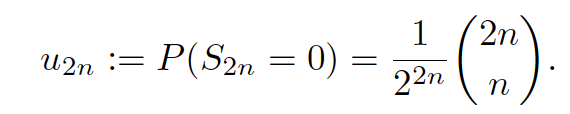
\includegraphics[scale=0.8]{WalkReturnToStartT2nProbability}
		\end{center}
		By \emph{Stirling's approximation}, it is
		\begin{center}
			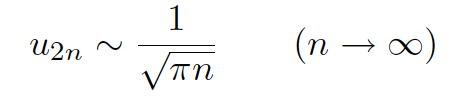
\includegraphics[scale=0.8]{WalkReturnToStartTnProbability}
			\cite{Durrett2010}
		\end{center}
	\item The walk eventually reaches each integer within $\mathbb{Z}$ lattice with certainty and so traverses it infinitely often. Suppose $S\textsubscript{0} := 0$ and $T := \inf\{n : S\textsubscript{n} = +1\}$ then $P(T < \infty) = 1$ and $P(T =  \infty) = 0$
	\item The distribution of \emph{T} is 
		\begin{center}
			$P(T = 2n - 1)\ =\ (-1)_{n-1}\binom{\frac{1}{2}}{n}$
		\end{center}
	\end{enumerate}
A Simple Random Walk generally refers to random walk in the first dimension. However, this research is concerned with random walks in 2 dimensions. But interestingly, a 2 dimensional random walk is essentially  composed of two Simple Random Walks in either plane as the vertices in either plane selected are independently selected.
\newline


\subsection{Loop Erased Random Walks (LERW)}
	A Loop erased random walk on the integer lattice is a process obtained from Random Walk by erasing the loops chronologically. In LERW, the process is expected to have a continuum limit that is conformal, and nonrigorous conformal, field theory gives an exact prediction of the exponent as a simple rational number. In three dimensions there is no reason to believe that the exponent takes on a rational value. Once the loops are erased from the random walk, it essentially becomes a uniform spanning tree (UST), which is a spanning tree chosen uniformly at random, and so the algorithms for generating LERWs are used in application to produce  uniform spanning trees.

\paragraph{Loop Erased Random Walk definition.} \label{alg:LE} If $\omega = [\omega\textsubscript{0}, \ldots, \omega\textsubscript{n}]$ is a path, then the \emph{(chronological) loop-erasure} function $LE(\omega)$ would be defined as follows\cite{klafter2011} \newline
	Let $\lambda_{0} = \max\{j\ \le \ n: \omega_{j}=0\}$. Set $\beta_{0}=\omega_{0}=\omega_{\lambda_{0}}$.
	\newline
	Suppose $\lambda_{i} < n$. Let $\lambda_{i+1} = \max\{j\ \le n: \omega_{j}=\omega_{\lambda_{i}+1}\}$. Set $\beta_{i+1}=\omega_{\lambda_{i+1}}=\omega_{\lambda_{i}+1}$.
	\newline
	If $i_{\omega} = \min \{i : \lambda_{i} = n\} = \min\{i : \beta_{i} = \omega_{n}\}$, then $LE\left(\omega\right) = \lbrack \beta_{0},\ldots,\beta_{i}\rbrack$
\newpage


\section{Methodology}
	In this section, I will explain the theory behind the code that was written to produce the resultant data. The code was mainly\footnote{The \emph{raw2binned.c} script in \texttt{C++} was used for the sake of efficiency and was originally written by Francesc, later modified by Gunnar Pruessner and then adapted by me for this project} written in \texttt{Python} as it enabled us to stay problem-oriented and allowed us to implement the LERW rapidly as well as readily provided us much greater useful functionality through its extensive library. I used the \texttt{matplotlib} library to generate the required statistical graphs from the data (i.e. distribution histograms) and \texttt{numpy} library to effective manipulate the data as well as conduct statistical analysis.


\subsection{Random Walk Implementation}
	The Random Walk was theoretically modelled to transverse on the 2 dimensional surface of a 3 dimensional cylinder (i.e. the system) with two vertical open boundaries and to two horizontal periodic. At the open boundaries, the  Random Walk is initiated from starting boundary and ceased at the ending boundary. Due to the curvilinear geometry of a cylinder, the system had the property of allowing the random walk to transverse an infinite number of steps in any vertical direction given that the random walk did not reach the ending boundary. 
The system was implemented as a 2 dimensional $\mathbb{Z}$ lattice of a particular size (length by circumference) which represented the 2 dimensional surface of the cylinder and, to implement the previously stated property of the original system, periodic boundaries where inaugurated. The function of the periodic boundaries was to ensure that the random walk continues to transverse from the boundary iteratively until it took a valid step (i.e. a step within the system boundaries) when the random walk surpassed a system boundary (see Figure~\ref{fig:RW}). The following is a formal definition of the system.

\paragraph{System definition.}\label{subsec:sysfdef} Given that $\vb{S}=\opair{i, j}$ is the system of size (L, C), where \emph{i} and \emph{j} are the respective vertical and horizontal components of the system (refer to Appendix~\ref{sssec:sysdef} for the actual system definition)
	\begin{enumerate}
		\item The system generation can be expressed as
			\begin{center}
				$\vb{S} = \left\{\left. (\sum_{k=0}^L i_k,  \sum_{k=0}^C j_k) \; \right\vert \;i_k j_k \in\mathbb{Z} \right\}$
			\end{center}
		\item The length and the circumference $(L, C)$ of the system are of equal size which implies that the lattice was of equal length (for this research)
		\item $\vb{S}\textsubscript{i = 0}$ is the starting boundary and $\vb{S}\textsubscript{i = L}$, where \emph{L}  represents the length of the system, is the ending boundary. 
		\item $(\vb{S}\textsubscript{i = 0}, \vb{S}\textsubscript{j = y})$  is the starting point, where \emph{y} is the first pseudorandom number in the sequence generated by lib function using a given seed.
		\item Periodic boundaries exist at $(\vb{S}\textsubscript{j = 0}, \vb{S}\textsubscript{j = C})$, where \emph{C} is the circumference of the system, to allow \emph{j} to be of an indefinite size
	\end{enumerate}

\paragraph{Random Walk generation.} A Random Walk, $S_{n}$, was generated using the generation function
	\begin{center}
		$\omega_{n} =  \sum_{k=0}^n X_k$
	\end{center}
where $\{X_k\}$ are independent and identically distributed random variables. 
Implementing the periodic boundaries as well, resulted in the generation function 
\begin{center}
		$\omega_{n} =  \left\{ \sum_{k=0}^n X_k \given[\Big] X_k \lnot\ 0 \lor L \lor C \right\}$
\end{center}
I translated this into \texttt{Python} code which is viewable in Appendix~\ref{sssec:srwgen}. In the code, the \emph{trajectory} list containing the running set of vertices corresponding to the pseudorandom steps that the random walk had talking was a \texttt{numpy} list because of extensive functionality (i.e functions/methods) that were required to perform the non trivial manipulations quickly as well as staying problem-oriented. For a plot of the random walk output of the generation code refer to the following figure (Figure~\ref{fig:RW}).
\begin{figure}
	\begin{center}
		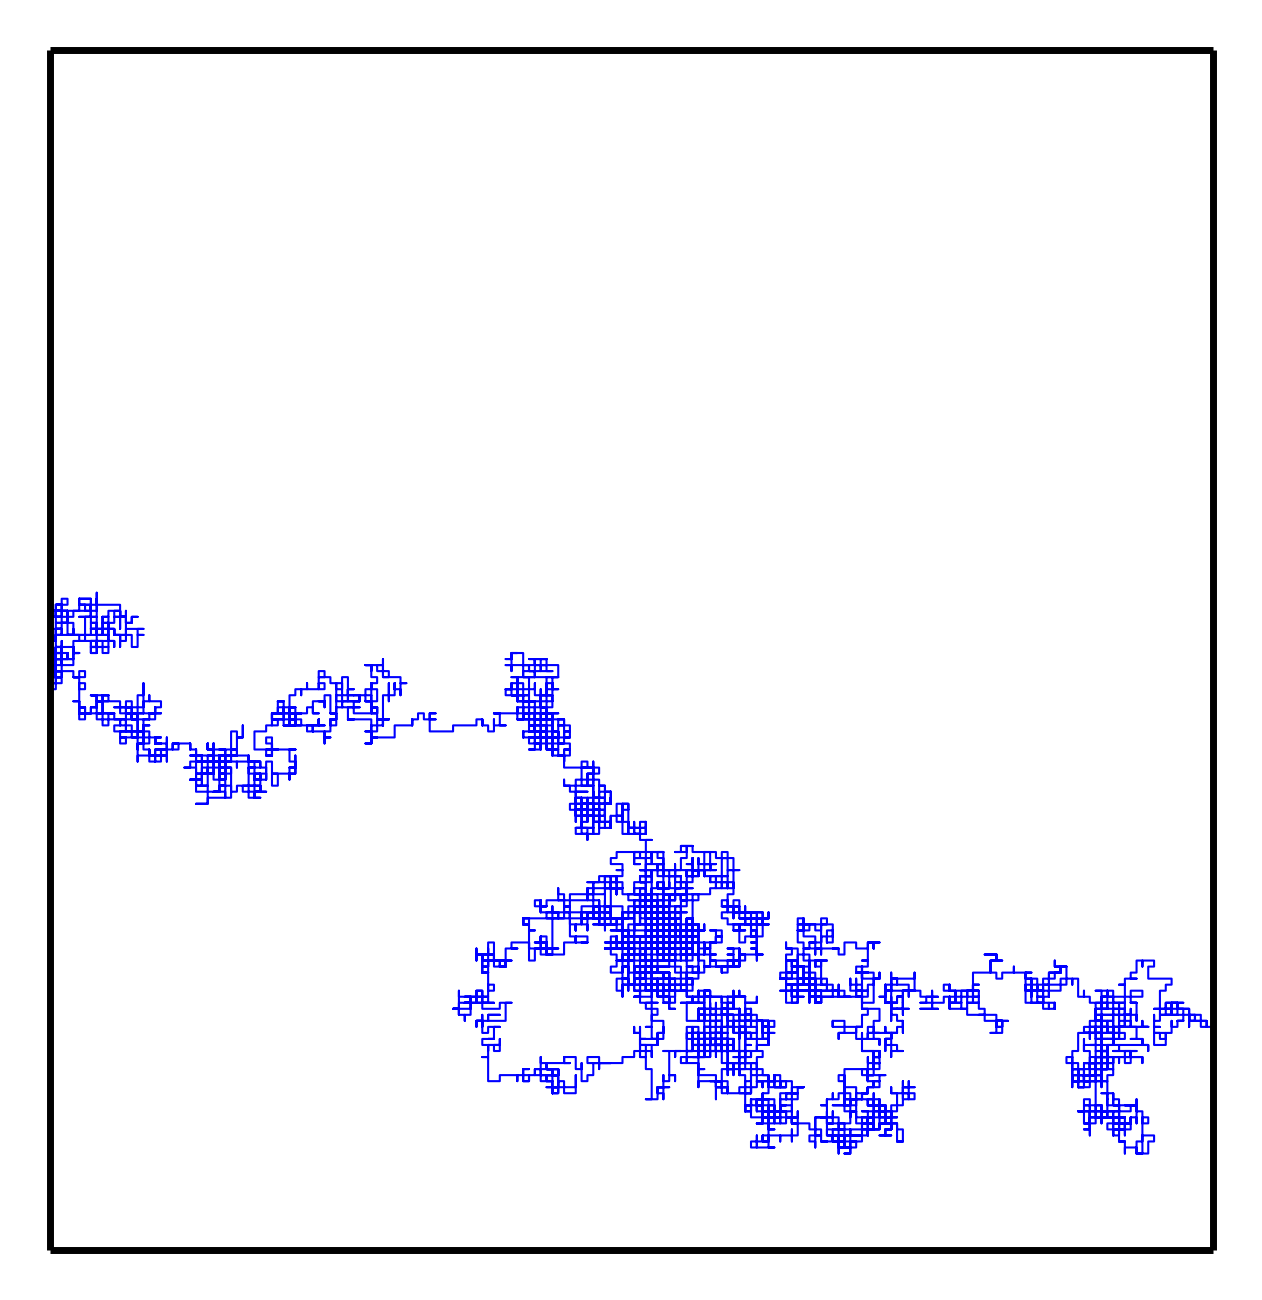
\includegraphics[scale=1.6]{RW_200s7hdpi}
		\caption{Random walk on a $\mathbb{Z}^{\emph{2}}$ lattice (system size: 200; seed: 7)}
		\label{fig:RW}
	\end{center}
\end{figure}

\paragraph{Random Walk Loop Erasure.} A loop is simply the result of the random walk intersecting itself. Considering that the random walk is transversing on an integer lattice, for a loop to occur, a vertex on the lattice has to be transversed at least twice - at the start of the loop and at the end of the loop. So to erase the loop, an algorithm was devised which removed every duplicate of a given list of vertices (i.e. the random walk trajectory) from the first occurrence of the vertex onwards to (and including) the last occurrence in the random walk trajectory list iteratively until all duplicates (i.e. loops) are removed. The $LE(\omega)$ algorithm defined in Loop Erased Random Walk definition in~\ref{alg:LE}, is a condensed form of the algorithm that was used to generate the LERWs to generate the data.
I translated this into \texttt{Python} code which is viewable in Appendix~\ref{sssec:lerw}. For a plot of the loop erased random walk output of the generation code refer to the following figure (Figure~\ref{fig:LERW}).
\begin{figure}
	\begin{center}
		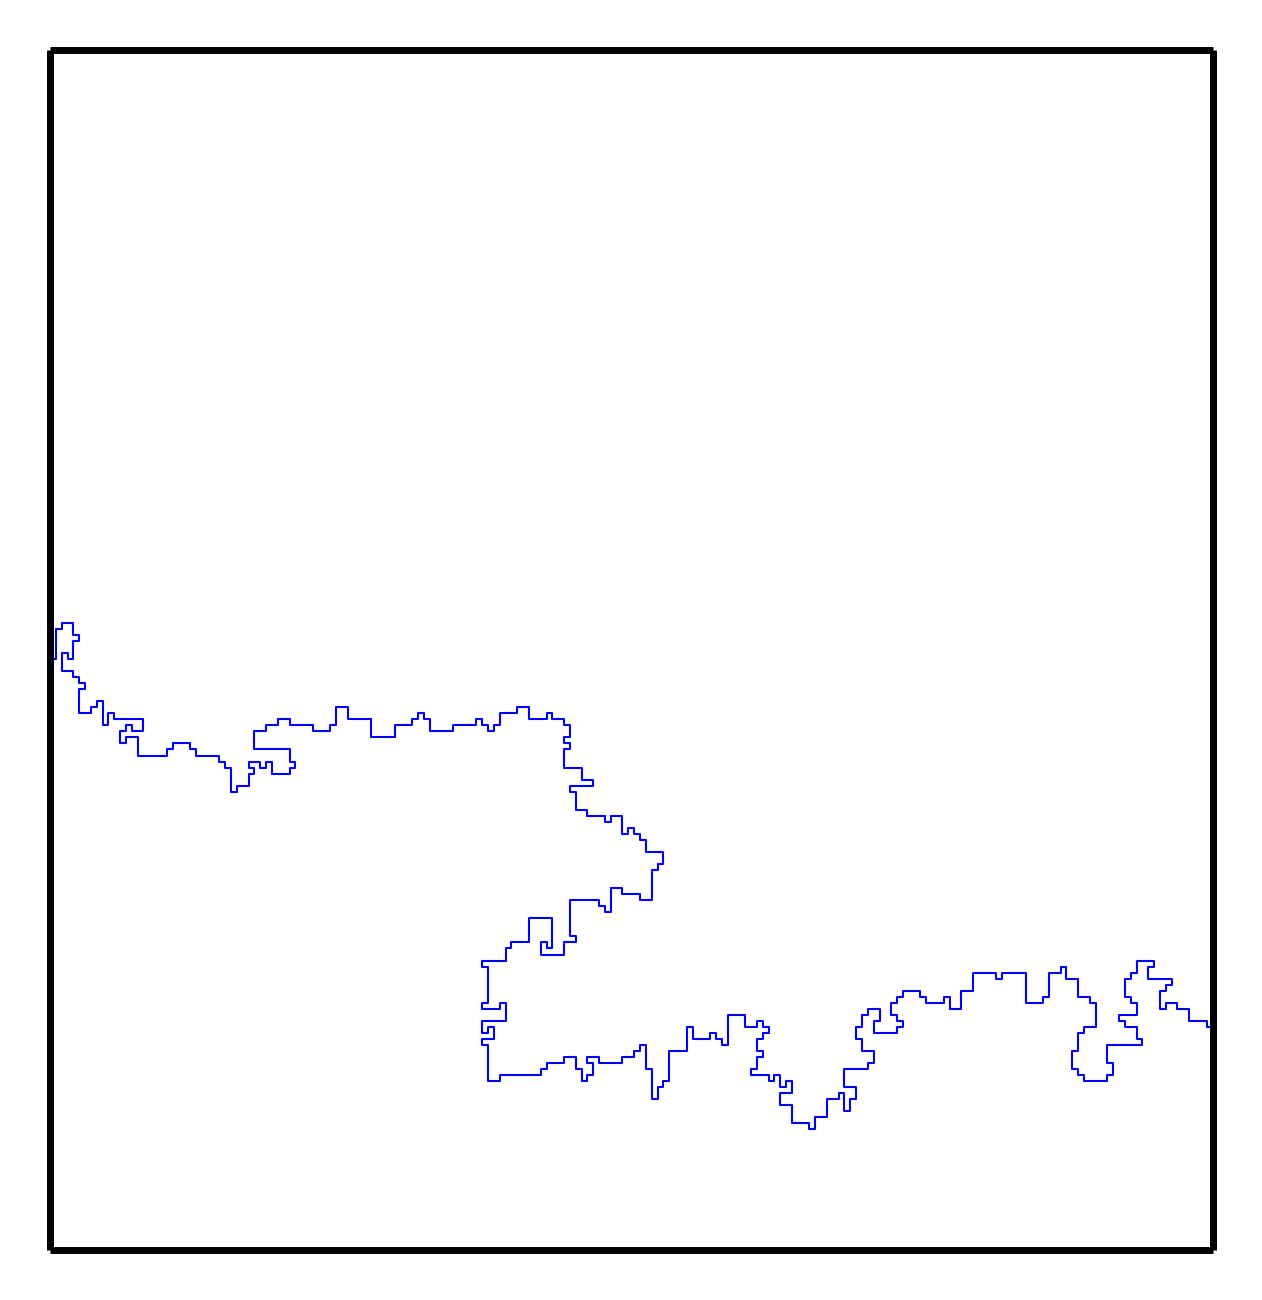
\includegraphics[scale=1.6]{LERW_200s7hdpi}
		\caption{Loop erased random walk on a $\mathbb{Z}^{\emph{2}}$ lattice (system size: 200; seed: 7)}
		\label{fig:LERW}
	\end{center}
\end{figure}
\newpage

\subsection{Data Collection}
	 All data collected for analysis was primary data generated by self-written code and systematic randomness.  Data collection was an automatic procedure carried out by the code that I had written when run. A significant amount data had to collected for different system in order to draw a reliable and a more decisive conclusion. As discussed before, the main implication of the presence of periodic boundaries was that the size of the vertical component was indefinite and thus the size of the result was indefinite. Since the code could not be optimised for multithreading, the task for the execution of the code could not utilise more than one core of the multi-core computational infrastructure. Also considering that the computational infrastructure was not dedicated for the task (i.e other OS-related task have had a higher priority), it was apparent that the code had to run for a prolonged period of time in order to collect the necessary. Data was collected for different systems, namely, one dimensional random walk,
\newline
Fortunately, the computational resource available at disposal for this project were vast. With access to the High Performance Computing (HPC) at Huxley Building, Imperial College London, the source code for generating the systems of various sizes was run as a series of jobs over the period of a whole day (~24 hours) to generate the data by the interpreter writing the output to a series of UTF-8 encoded sequential .dat files. Some metadata (such as the system size) was prepended to the files to distinguish and identify the files easier.
\newline
Data was collected for the following systems:
\begin{itemize}
	\item 2 dimensional Random Walks of system sizes of 50, 100, 200 and 400
	\item 1 dimensional Random Walks of system sizes of 50, 100, 200 and 400
	\item 2 dimensional Loop Erased Random Walks of system sizes of 50, 100, 200 and 400
\end{itemize}
On the first run on the cluster, we received a runtime error due to the incorrect configuration of the cluster but this was quickly fixed once the system was reconfigured. Once the files containing the data were generated, they were inspected manually to ensure that the generated data was valid (i.e. conformed to the expected data) and no logical errors where present in the code. Due to time constraints for each job of 15 hours on the cluster and considering that only one core of the cluster was being utilised, the code for generating the 2 dimensional Random Walks of system sizes of 400 and the code for generating 2 dimensional Loop Erased Random Walks of system sizes of 200, 400 was unable to completely execute. This incomplete execution resulted in the files not being generated (files were not completely written and so any associated temporary was discarded).
Hence, \emph{in this report we will only analyse the data by a system\footnote{refer to \S~\ref{subsec:sysfdef} for definition} where} $|\vb{S}| \le 200$ .\newline
These outputs where then run through the \emph{raw2binned.c} script that grouped the raw data into bins in order to plot a double logarithmic histogram (refer to Results and Analysis to see the resulting plot).
\newpage
	

\section{Results and Analysis}
	The collected data was used to generate plot double logarithmic histograms (refer to Figure~\ref{fig:LERWhdish} -~\ref{fig:RW2Dhdish}) in order to qualitatively compare the return times distributions for 2 dimensional discrete ($\mathbb{Z}^{\emph{2}}$) LERWs,  2 dimensional discrete ($\mathbb{Z}^{\emph{2}}$)  Random Walks and 1 dimensional discrete ($\mathbb{Z}$) Random Walks. \newline

What my research found was that was that return times distribution for $\mathbb{Z}^{\emph{2}}$ random walk and return times distribution for $\mathbb{Z}$ random walk were very similar. What my research also found that there is a difference in the distribution of the return times of a random walker (1D and 2D)  and the distribution of the loops erased in LERW.

\paragraph{Return distribution of 1D and 2D Random Walks.} Comparing Figure~\ref{fig:RW1Dhdish} and Figure~\ref{fig:RW2Dhdish}), I found that the return times distribution for $\mathbb{Z}^{\emph{2}}$ random walk and return times distribution for $\mathbb{Z}$ random walk were very similar. The following is a possible explanation for this discovery that implicates a significant amount of factual knowledge in the field. For a random walk in one dimension starting at $n$, the probability that the random walk eventually returns to $n$ equals one \cite{Redner2002} $\implies \Pr(S_{n}=n) = 1$, $n \in \mathbb{Z}$. However, the time required to return to $n$, averaged over all possible vertices in the system, is infinite.For a random walk in two dimensions, the survival probability $S(t)$ ultimately decays to zero. This means that a random walk is recurrent which means that it is certain to eventually return to its starting point, and indeed visit any vertex of an infinite lattice. This is the $2.$ deduced characteristic stated in $\S1.1$.  This is also because a random walk has no memory and so it transits to a new state (i.e. resets it\' s state) every time a specific lattice vertex is transversed. Hence, recurrence also implies that every site is visited infinitely often.
The arcsin law, which is concerned with the statistics of returns to the origin, also applies here as our random walk is an unrestricted random walk. From the arcsine law, we can infer that the most probable outcome is that the walk always remains entirely on the positive or on the negative axis. This is against the natural expectation of approximately one-half of the total time being spent on the positive axis and the remaining one-half of the time on the negative axis for a random walk which starts at x = 0. Surprisingly, the natural expectation is the least probable outcome.
\paragraph{Difference in arc length distribution of returns and loops erased.} As depicted in Figure~\ref{fig:AREr}, there is a correlation between the distribution of the loops erased in a random walk and the probability of return to (an arbitrary) vertex in the lattice for both systems of size 100 and 200. In fact, the combined distribution is positively skewed which implies that as the loops erased increase, the probability of returning to a vertex in the lattice decreases. The fact that the data is skewed, indicates that there is a difference arc length distribution of a random walker returning and arc length distribution of the loops erased.
\newpage

\begin{figure}[H]
	\centering
		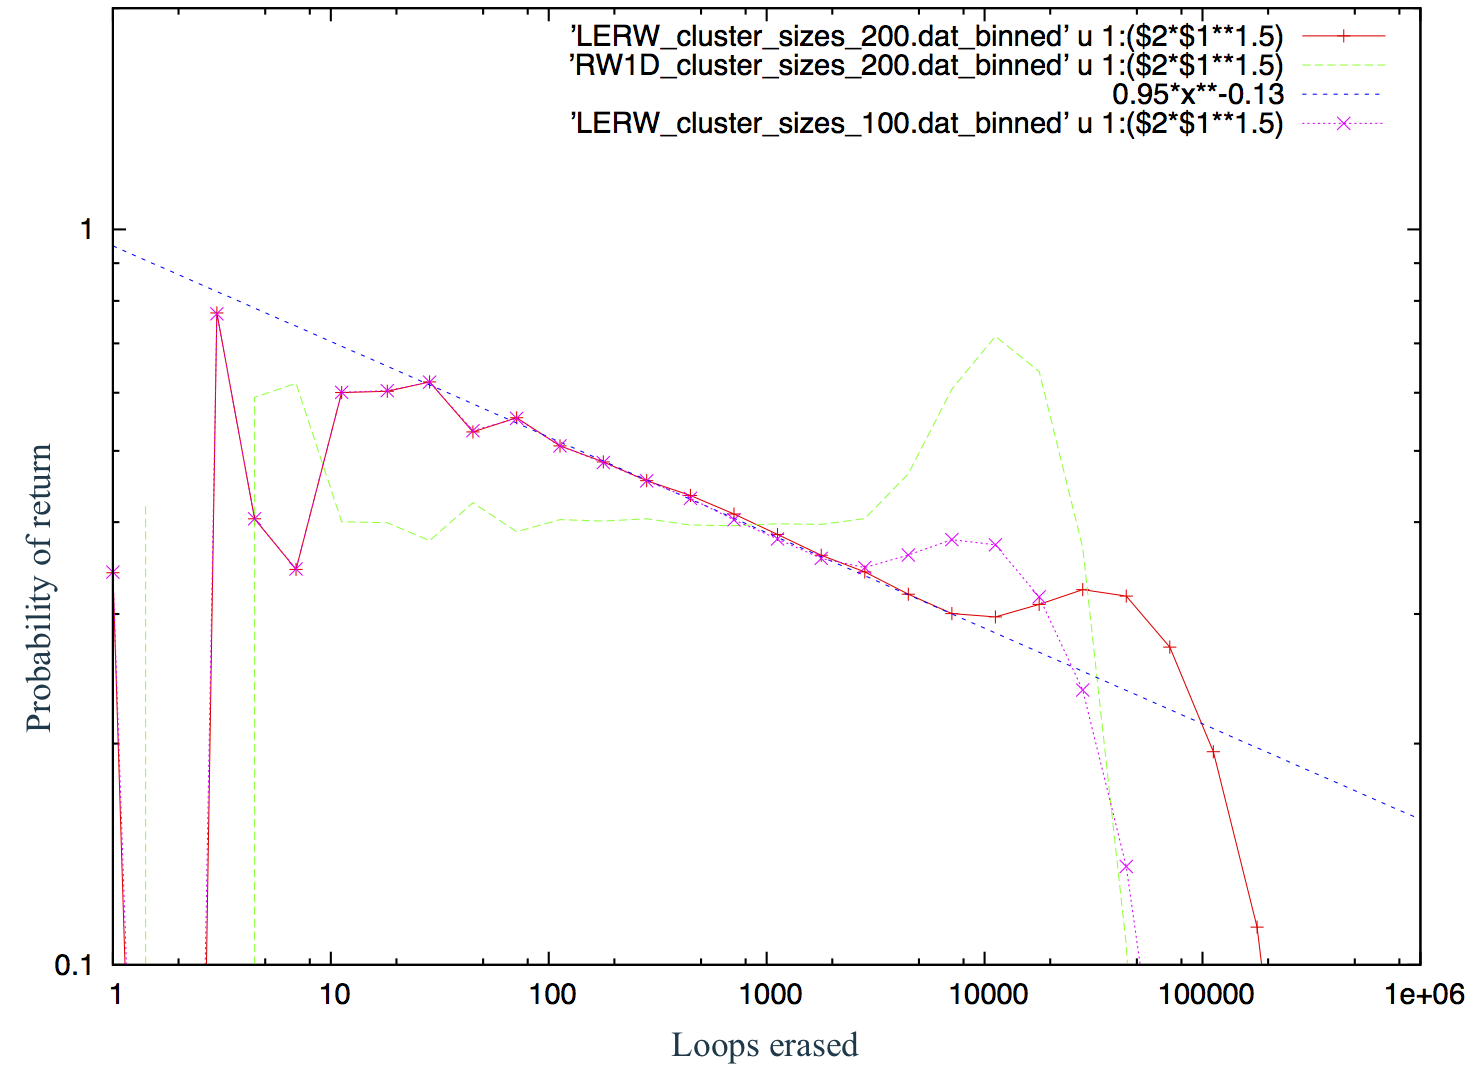
\includegraphics[scale=0.6]{preturn_le_plot}
		\caption{Probability of return and loops erased distributions for $\mathbb{Z}^{\emph{2}}$ LERWs (system sizes: 100, 200; seed:10) and $\mathbb{Z}$ Random Walk (system size:200; seed:10)}
		\label{fig:AREr}
\end{figure}
\begin{figure}[H]
	\centering
		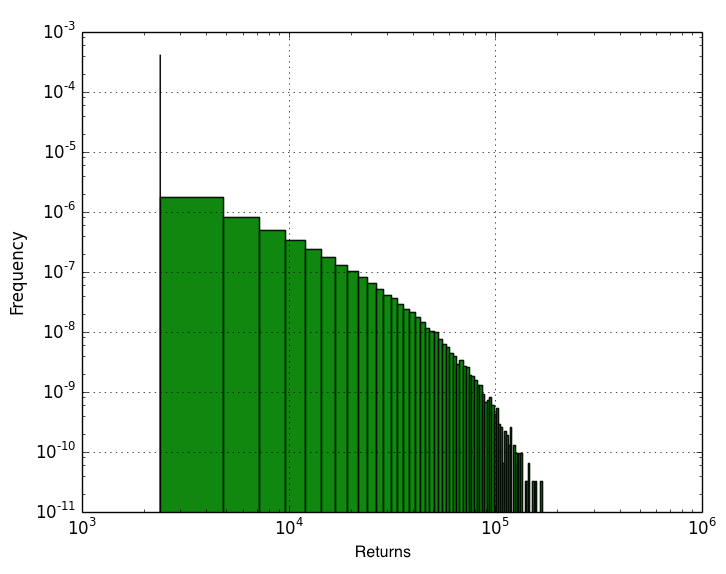
\includegraphics[scale=0.5]{LERW_cluster_sizes_200_histogram}
		\caption{Histogram for the distribution of the Loop Erased for Random Walks on $\mathbb{Z}^{\emph{2}}$ lattice (system size:200; seed:10)}
		\label{fig:LERWhdish}
\end{figure}
\begin{figure}[H]
	\centering
		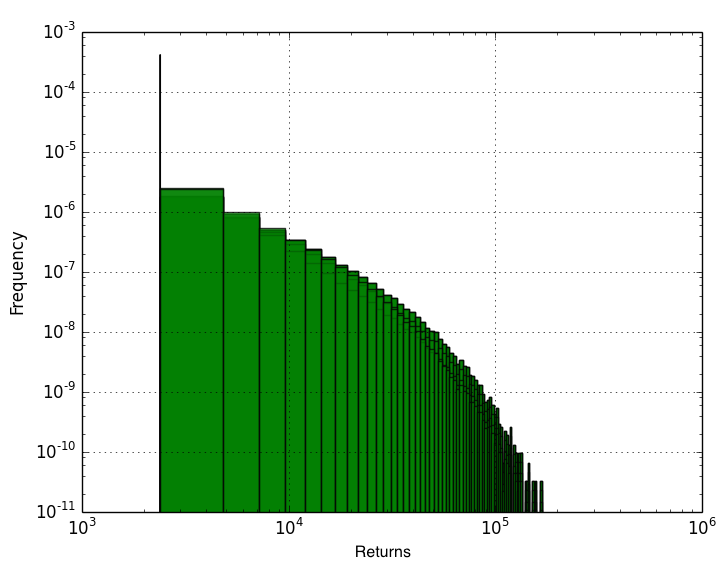
\includegraphics[scale=0.5]{RW1D_cluster_sizes_200_histogram}
		\caption{Histogram for the returns distribution of Random Walks on $\mathbb{Z}$ lattice (system size:200; seed:10)}
		\label{fig:RW1Dhdish}
\end{figure}
\begin{figure}[h]
	\centering
		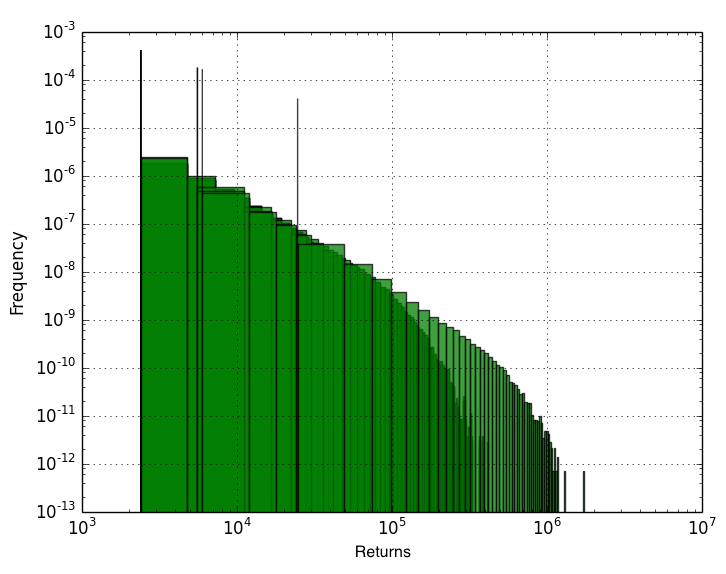
\includegraphics[scale=0.5]{RW2D_cluster_sizes_200_histogram}
		\caption{Histogram for the returns distribution of Random Walks on $\mathbb{Z}^{\emph{2}}$ lattice (system size; seed:10)}
		\label{fig:RW2Dhdish}
\end{figure}
\newpage

\section{Conclusion}
The research has correspondence between the return distribution of a one-dimensional random walk and a two- dimensional random walk. I can conclude that similarity in the return distribution of the one-dimensional random walk and the two-dimensional random walk is due to the survival probability of the two-dimensional random walk eventually being zero and we know that the probability of a one-dimensional random walk is already one. We can also conclude that there is a difference in the distribution of the return times of a random walker and the distribution of the loops erased in LERW. \newline

This research can be extended by using Self Avoiding Random Walks (SARW) which are random walks that do not self-intersect during their transversal and are in a different universality class from LERW.


\section{Appendices}
	\emph{Please note that the all the code (listed separately here as sections) is part of the same source code file unless stated otherwise. Hence, any variables/constants declared are accessible throughout the (5.x) code sections respectively of their scope.}
	\subsection{System Definition code} \label{sssec:sysdef}
	\lstinputlisting[language=Python]{pysc/sysdef.py}
	\subsection{Random Walk generation code} \label{sssec:srwgen}
	\lstinputlisting[language=Python]{pysc/srwgen.py}
	\subsection{Loop Erased Random Walk code} \label{sssec:lerw}
	\lstinputlisting[language=Python]{pysc/lerw.py}


\section{Bibliography}	
	\bibliographystyle{amsplain}
	\bibliography{references}
	

\section{Acknowledgements}
I would like to thank Professor Gunnar Pruessner of Imperial College London for supervising the research project and the Nuffield Foundation for funding this research. I would also like to thank Imperial College London for allowing us to use the High Performance Computing (HPC) mainframes at Huxley Building in ICL.
\end{document}